\documentclass{article}
\usepackage[utf8]{inputenc}
\usepackage{graphicx}

\begin{document}
\begin{center}
\large\bfseries{Washing Machine Status Tracker}
\end{center}
\begin{center}
\vspace*{1.2cm}
\noindent \textbf{DBMS PROJECT}

\noindent \textbf{PHASE 1}
\vspace*{1.2cm}

\noindent By

\noindent \textbf{T.S.M THRIVEEDH} - CS22B1010

\noindent \textbf{B.SIDDHARTHA REDDY} - CS22B1099

\noindent \textbf{T.SAI MADAN} - CS22B2023

\noindent \textbf{G.SRI RAM} - CS22B2020

\noindent \textbf{H.SAI SANDEEP} - CS22B2019

\end{center}
\begin{figure}[h]
\begin{center}
\end{center}
\end{figure}
\newpage
\tableofcontents
\newpage

\section{Introduction}
\subsection{Purpose}
This project allows students to efficiently manage their laundry without disturbing their schedules,reducing waiting time by being the one-stop solution for all laundry problems.
Automation ensures that washing machines are utilized optimally,ensuring smooth operation for all users.
\subsection{Intended Audience}
This project is particularly beneficial for hostel and PG students,catering to environments where the number of washing machines is limited compared to the high demand among the student population.
\subsection{Project Scope}
This project is aimed at providing students with real-time updates on the status of individual washing machines, making it easier for them to see which ones are available whenever they need to do their laundry. 

Additionally, there will be an administrative dashboard specifically designed for authorized personnel. This dashboard will allow them to update the status of the washing machines and handle any complaints that may arise.  

It's worth mentioning that this project won't include any advanced features like booking systems or remote-control capabilities for the machines. 
\section{Overall Description}
\subsection{Functional Requirements}
\begin{itemize}
\item\textbf{User Authentication and Authorization:} 

The system shall provide user authentication mechanisms to verify the identity of users accessing the system. Authorized users, such as staff and administration, shall have specific roles and permissions to perform certain actions within the system. 

\item\textbf{User Logging:}

The system shall log user interactions with the washing machines to maintain usage history. User interactions to be logged include the student's roll number and the machine ID they are using.  

The logged information shall be stored securely and tamper-proof to ensure data integrity and traceability. Access to user logs shall be restricted to authorized personnel, such as administration and system operators.

\item\textbf{Real-time Monitoring:}

The system shall continuously monitor the status of each washing machine in real-time, including availability, current usage, and maintenance status. 

\item\textbf{Admin Interface:}

The administrative dashboard shall provide authorized personnel with the ability to manage washing machine information and update statuses. Admins shall have the capability to view user log details.

\end{itemize}
\subsection{Non-functional Requirements}
\begin{itemize}
\item\textbf{Performance:}

The system must efficiently handle concurrent requests from multiple users without experiencing significant performance degradation. 

\item\textbf{Availability:}

The system should be available for use 24/7 with minimal planned downtime for maintenance or updates, ensuring uninterrupted service for users. 

\item\textbf{Security:}

Robust security measures must be implemented to protect user information. This includes the implementation of authentication and authorization mechanisms to control access to system resources and safeguard sensitive data. 

\item\textbf{Usability:}

The user interface must be intuitive and user-friendly, featuring clear navigation and layout to facilitate ease of use for all users. This includes providing straightforward access to features and functionalities to enhance the overall user experience. 

\item\textbf{Maintainability:}

The system should be designed with modular and well-documented code to facilitate ease of maintenance and accommodate future enhancements. This ensures that updates and modifications can be made efficiently without compromising system integrity or functionality. 

\item\textbf{Compatibility:}

The system is designed to support common web browsers and ensures seamless compatibility across a variety of platforms, ensuring accessibility and usability for all users, regardless of their preferred device or operating system.  
\end{itemize}

\section{System Features}
\subsection{Technology Stack}
Our tech stack includes SQL (MySQL), JavaScript, HTML, and CSS, complemented by node.js with express.js for backend development. 
\subsection{System Requirements}
\begin{itemize}
\item Works on any operating system.

\item Internet connection is required. 

\item Works on any browser.
\end{itemize}

\begin{figure}
\begin{center}
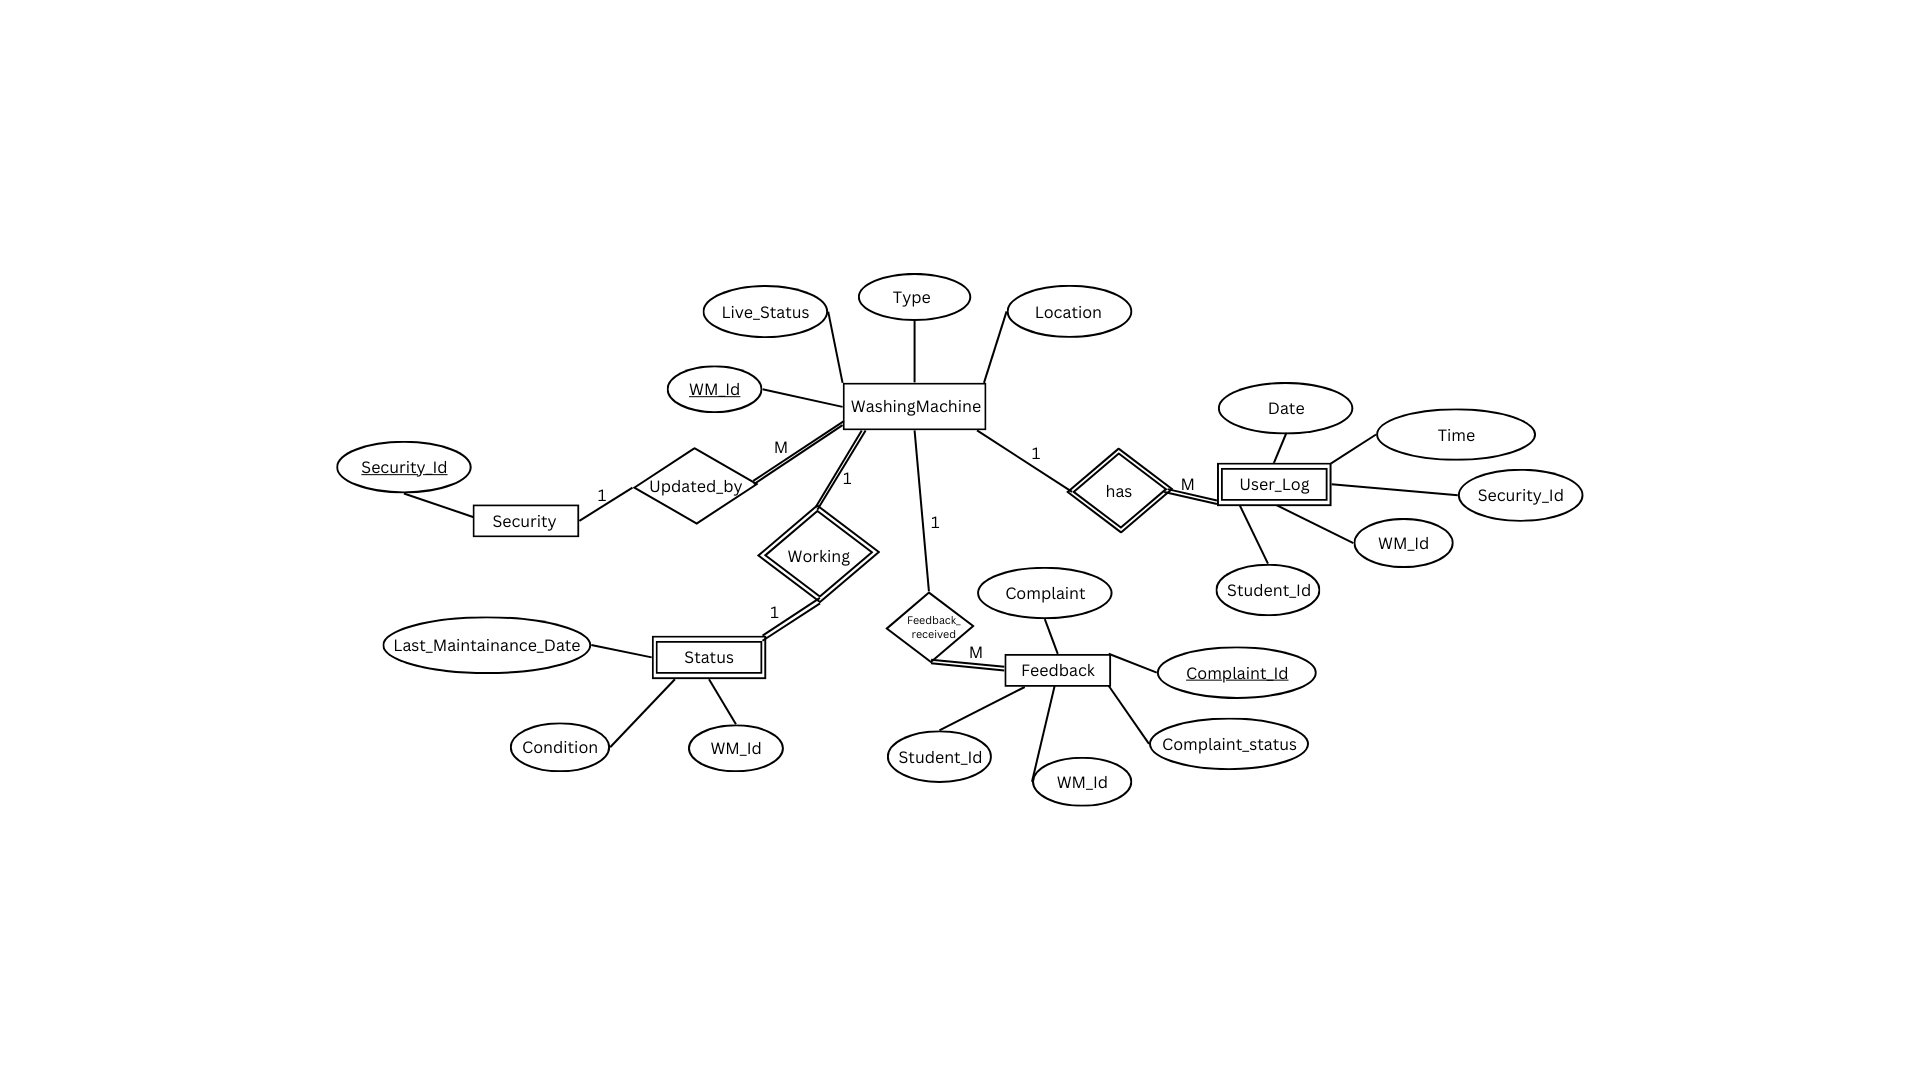
\includegraphics[width=1\textwidth]{dbms2.jpg}
\end{center}
\caption{ ER-Diagram}

\end{figure}
\begin{figure}
\begin{center}
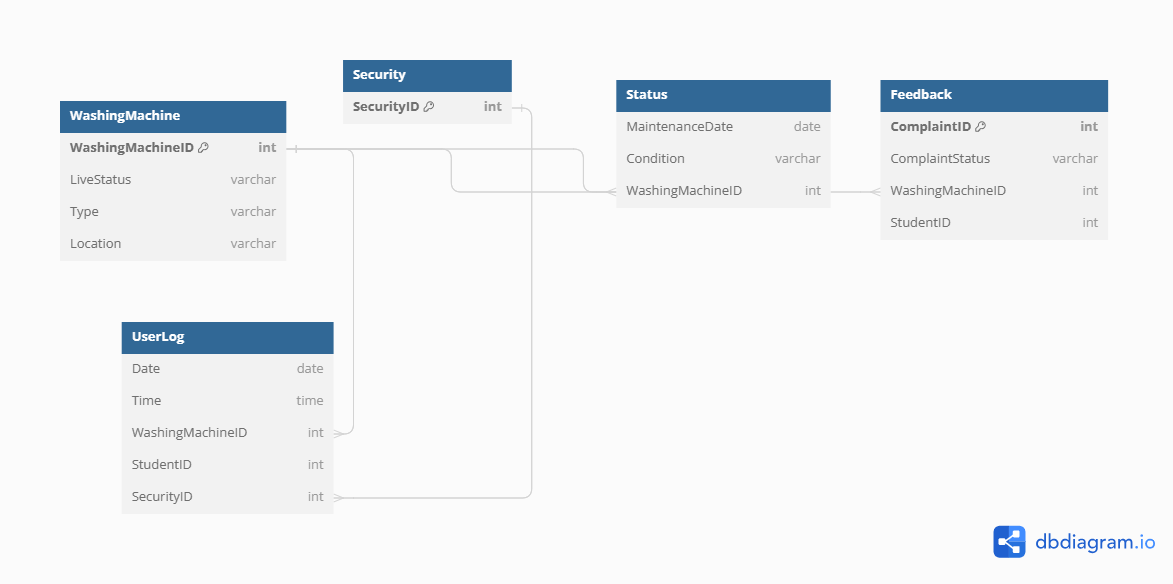
\includegraphics[width=1\textwidth]{dbms1.jpg}
\end{center}
\caption{ Schema}

\end{figure}

\end{document}
